\documentclass[a4paper, 12pt]{article}

\usepackage{lmodern}
\usepackage{indentfirst}
\usepackage[utf8]{inputenc}
\usepackage{authblk}
\usepackage{fancyhdr}
\usepackage{setspace}
\usepackage{graphicx}
\usepackage{hyperref}
\usepackage{booktabs}
\usepackage{titlesec}
\usepackage[usestackEOL]{stackengine}
\usepackage{float}
\usepackage{adjustbox}
\usepackage[tableposition=top]{caption}
\usepackage{systeme}
\usepackage{amsmath}
\usepackage{mathtools}
\usepackage{commath}
\DeclareUnicodeCharacter{200A}{!}

\usepackage[
 left=31.7mm,
 top=25.4mm,
 right=31.7mm,
 bottom=25.4mm
]{geometry}

\usepackage[style=abnt, pretty, usedashes, doi=false, hyperref=false, url=false, isbn=false, eprint=false,  language = english]{biblatex}
\addbibresource{master_mutantag.bib} 

\AtEveryBibitem{%
  \clearfield{note}%
}

\usepackage{microtype}

\renewbibmacro*{name:andothers}{% Based on name:andothers from biblatex.def
  \ifboolexpr{
    test {\ifnumequal{\value{listcount}}{\value{liststop}}}
    and
    test \ifmorenames
  }
    {\ifnumgreater{\value{liststop}}{1}
       {\finalandcomma}
       {}%
     \andothersdelim\bibstring[\emph]{andothers}}
    {}}

\titleformat{\section}{\centering\large}{}{0em}{\MakeUppercase}[\titlerule]

\renewcommand{\contentsname}{Índice}

\newcommand*\wildcard[2][5cm]{\vspace*{2cm}\parbox{#1}{\hrulefill\par#2}}

\renewcommand\Authfont{\fontsize{14}{14.4}\selectfont}
\renewcommand\Affilfont{\fontsize{10}{10.8}\itshape}

% Title and authors
\title{\vspace{-2.0cm}\textbf{Coevolutionary exploitative interactions increase trait disparity and modularity in mutualistic networks}}

\author[1,*]{Lucas Arantes Camacho}
\author[2]{Cecilia Siliansky de Andreazzi}
\author[3]{Lucas Paoliello Medeiros}
\author[4]{Irina Birskis Barros}
\author[5]{Carine Emer}
\author[6]{Carolina Reigada Montoya}
\author[7]{Paulo Roberto Guimarães Junior}
\affil[1]{Programa de pós graduação em Ecologia, Departamento de Ecologia - Instituto de Biociências, Universidade de São Paulo, USP, Rua do Matão, Tv. 14 - Butantã, São Paulo - SP, 05508-090}
\affil[2]{Instituto Oswaldo Cruz (IOC/FIOCRUZ), Avenida Brasil, 4365 - Manguinhos. Rio de Janeiro, RJ, Brasil}
\affil[3]{Department of Civil and Environmental Engineering, MIT, 77 Massachusetts Ave, 02139 Cambridge, MA, USA}
\affil[4]{School of Natural Sciences, University of California, Merced, EUA}
\affil[5]{Centro Nacional de Pesquisa e Conservação de Aves Silvestres (CEMAVE). BR 230 - KM 10. Floresta Nacional da Restinga de Cabedelo, Renascer.  Cabedelo - PB Brasil}
\affil[6]{Centro de Ciências Biológicas e da Saúde da UFSCAR, Departamento de Ecologia e Biologia Evolutiva - São Carlos, SP - Brasil}
\affil[7]{Departamento de Ecologia - Instituto de Biociências, Universidade de São Paulo, USP, Rua do Matão, Tv. 14 - Butantã, São Paulo - SP, 05508-090}
\affil[*]{\textbf{corresponding author: lucas.camacho@usp.br}}
\date{}

% Begin document
\doublespacing
\begin{document}

\setcounter{page}{1}
\begin{center}
\begin{Huge}
Lucas Arantes Camacho

\topskip0pt
\vspace*{\fill}
\begin{singlespace}
Coevolução e exploração em redes de mutualismos \\
\vspace{10pt}
Coevolution and exploitation in mutualistic networks
\end{singlespace}

\end{Huge}
\end{center}

\begin{flushright}
\begin{minipage}{15em}
\begin{singlespace}
Dissertação apresentada ao Instituto de Biociências da Universidade de São Paulo, para a obtenção de Título de Mestre em Ciências, na área de Ecologia.
\bigbreak
Orientador: Prof. Dr. Paulo Roberto Guimarães Junior
\end{singlespace}
\end{minipage}
\vspace*{\fill}
%
\end{flushright}

\begin{center}
\vfill
São Paulo

2020
\end{center}

\newpage

\section*{Ficha catalográfica}

\begin{center}
\vspace{10mm} %5mm vertical space
\fbox{\begin{minipage}{30em}
Camacho, Lucas Arantes.
	Coevolução e exploração em redes de mutualismos.
	55 páginas.

	Dissertação (Mestrado) - Instituto de Biociências da Universidade de São Paulo. Departamento de Ecologia.

	1. Coevolução  2. Disparidade de traços  3. Mutualismos 4.Pilhadores 5. Teoria de redes  I. Universidade de São Paulo. Instituto de Biociências. Departamento de Ecologia.
\end{minipage}}
\bigbreak
\textbf{Comissão Julgadora:}

\begingroup
  \centering
  \wildcard{Dr(a).	}
  \hspace{1.5cm}
  \wildcard{Dr(a).	}
  \par
\endgroup

\begingroup
  \centering
  \wildcard{Dr(a).	}
  \hspace{1.5cm}
  \wildcard{Orientador}
  \par
\endgroup

\vspace*{\fill}

\end{center}
\newpage

\section*{Dedicatória}
 \thispagestyle{plain}
{\raggedleft\vfill\itshape\Longstack[l]{%
  \textit{Para minha mãe Mirna,}\\
  \textit{e minha vó Nadyr}\\
}\par
}
\newpage

\section*{Epígrafe}
\thispagestyle{plain}
\vfill
 
Um ecossistema se trata de um sistema. Um sistema!
Um sistema mantém certa estabilidade fluída que pode ser destruída por um deslize em apenas um nicho.
Um sistema tem ordem, uma correnteza que flui de um ponto a outro.
Se algo represar a correnteza, a ordem desmoronará.
Os inexperientes talvez só percebam esse desmoronamento quando já for tarde demais.
É por isso que a função mais elevada da ecologia é a compreensão das consequências.

\begin{flushright}
Pardot Kynes, o primeiro planetólogo de Arrakis

(Frank Herbert. \textbf{Duna}. São Paulo: Aleph, 2017)
\end{flushright}
\newpage

\section*{Agradecimentos}
 \thispagestyle{plain}
Muitas pessoas são responsáveis por esse documento existir. Pessoalmente eu posso tentar, mas acho difícil que essa seção dê conta de mostrar o quanto essas pessoas me apoiaram e transformaram a pós graduação em um lugar aberto, tranquilo e cheios de ciência que te faz querer saber um pouquinho mais sobre qualquer coisa. São essas pessoas que eu me refiro. Primeiro eu queria agradecer ao Miúdo, por ter aceito um terceiro Lucas no laboratório em 2015 e desde lá, me ajudado e me guiado nesse aprendizado. Obrigado também por compartilhar seu amor pela natureza e vontade de resolver quebra cabeças (até resolver um desses comigo, nascendo uma dissertação de mestrado cheia de resultados legais). Obrigado mesmo. Por tudo. Posso ir pra outros lugares continuar meu aprendizado, mas já me sinto com muita sorte de ter começado contigo e as coisas que aprendi contigo, levarei pra sempre. Espero poder estar sempre por perto, até porque tem livros de ciência seus que estão comigo ainda :)

A todos os integrantes e ex-integrantes do MiudoLab que me receberam com tanto carinho como o Lucas III e tornaram esse laboratório um ambiente tão divertido. Irina, Marília, Paulinha Lemos, Paulinha Assis, Flávia, Cecília, Roberta, Rafael, Taio, Pato, Pinguim, Anna, Coraline, Dani, Pammm, Pamela F., Leandro, Andres, Débora, Kate, Danilo e mais outras tantas pessoas que passaram rapidinho pelo laboratório. Espero que ele continue sempre assim e que eu possa voltar sempre que possível pra tomar um café com vocês no puxadinho. A verdade é que tenho sentimentos conflitantes em relação a sair do laboratório e se esse sentimento existe, significa que valeu muito a pena. Obrigado de verdade a todos vocês por formarem uma casa com relações tão boas.

Todos os dias eu trabalhei em uma sala cheia de pessoas com interesses muito diferentes mas que sempre foram muito carinhosas comigo. A todas as pessoas da LAGE e dos laboratório vizinhos. Muito obrigado. Glauco, Edu e PI, muito obrigado por estarem sempre presentes na LAGE e por fomentarem esse ambiente alegre e cheio de boas distrações para o trabalho. Obrigado aos alunos e alunas desses laboratórios que deixaram muito dos meus dias melhores e mais animados e mesmo que menos produtivos, no fim o trabalho está feito e está todo mundo feliz.

Agradeço especialmente ao Gustavo Burin e ao Marco Mello por terem aceitado fazer parte do meu comitê e terem me ajudado de tantas formas ao longo desses dois anos. Uma parte do que está aqui veio de conversas com vocês na sala 250 sobre redes, ecologia e evolução. Só tenho a agradecer por ter tido contato com pessoas tão incríveis.

Também agradeço as pessoas que fizeram parte desse trabalho comigo e me ajudaram no processo de escrita, em criticar  e pontuar novos caminhos para o meu trabalho. Esse artigo será uma colaboração de diversas pessoas e todas elas me ensinaram um pouco de ser cientista. Obrigado Lucas Medeiros, Irina Barros, Cecília Andreazzi, Carine Emer, Carol Reigada e Miúdo.

Além disso, a Ecologia me trouxe mais do que uma dissertação. Me ensinou a fazer um projeto de pesquisa e orientar alunos. Obrigado a todos e todas da comissão da EcoEscola 2019 por terem feito o que ela foi. Na real, me senti mais próximo de muitas pessoas do departamento com a EcoEscola e acho que esse foi um dos maiores ganhos. Obrigado a todos e se você estiver lendo isso e pertencer ao Dep. De Ecologia da USP: participe da EcoEscola. 

No primeiro ano de mestrado eu tive a chance de ir para a Amazônia e participar da experiência mais intensa e surreal da minha vida, além de pegar avião pela primeira vez. Obrigado a toda a organização do EFA e por terem me dado a oportunidade de aprender tanto com vocês. Obrigado. Além disso, um agradecimento especial ao Glauco que me deu dicas de como sobreviver na Amazônia e aproveitar o máximo do curso. Obrigado pelas dicas.

Aos funcionários do departamento de Ecologia da USP que foram sempre amigáveis e topavam uma conversa nos encontros casuais na copa ou pelos corredores. Muito obrigado pela ajuda com os problemas burocráticos/técnicos do dia-a-dia mas que vocês deixaram tudo um pouco mais leve. Meu muito obrigado.

Queria agradecer minha família do fundo do meu coração, por me incentivar sempre a estudar e por me apoiarem. Tia Cristina, Bianca, Camillinha e todo o resto da família. Mesmo que não fique tão claro o que eu faço ou o que eu quero fazer na ciência, tenho certeza que vocês apoiarão e isso é precioso demais para mim. Mãe e Vó, essa dissertação é pra vocês. Obrigado por me apoiarem e estarem sempre, desde criança, lendo perto de mim. Não sei direito como explicar como isso me influenciou a chegar aqui, mas sei que foi importante. Só muito obrigado e amo muito vocês.

Esse mestrado não teria sido igual se não fosse pelo meus amigos da graduação me apoiando e escutando minhas reclamações as vezes. Anna, Ju e Paulo, muito obrigado por estarem presentes e comigo. Amo vocês. Tenho muita sorte de ter bons amigos por perto.

O mestrado não me trouxe somente aprendizado sobre ciência. Joice, muito obrigado por ter topado ser minha companheira nessa jornada doida que é a vida. A gente já dividiu tanta coisa e você viu de perto o quanto tem de mim nessa dissertação. Obrigado pelo amor e pelo apoio de sempre. Te amo.

Finalmente, quero agradecer ao CNPq (Processo 130804/2018-5, 03/2018 a 02/2020) que pagou minha bolsa de mestrado ao longo de dois anos para que eu estudasse em tempo integral, o corpo de funcionários do IB e a USP por me aguentar como aluno por todo esse tempo.

\newpage

\tableofcontents
\newpage

\newrefsection
\thispagestyle{plain}
\addcontentsline{toc}{section}{Coevolutionary exploitative interactions increase trait disparity and modularity in mutualistic networks}
%\section*{Do we split or we merge? Exploitative interactions increase trait disparity and modularity through coevolution in mutualistic networks}

\begin{singlespace}
\maketitle
\end{singlespace}
\newpage

\addcontentsline{toc}{subsection}{Resumo}
\subsection*{Resumo}
Interações entre indivíduos de espécies diferentes formam, em uma localidade, redes de interações. Nessas redes, mudanças adaptativas podem gerar efeitos indiretos, podendo levar a novas dinâmicas evolutivas. Estas novas dinâmica evolutivas podem ser influenciadas por interações que apresentam consequências distintas para a aptidão dos indivíduos interagentes. Por exemplo, em mutualismos, redes de interações emergem que podem favorecer a evolução de modos de vida que apenas exploram indivíduos mutualistas sem fornecer benefícios e, por conseguinte, reduzem a aptidão dos indivíduos explorados. Aqui, estudamos como a exploração e seus diferentes padrões de interação influenciam a dinâmica coevolutiva em redes mutualistas. Combinamos  um modelo coevolutivo para redes ecológicas, dados sobre redes empíricas de mutualismos e simulações numéricas para sugerir que a presença de exploração aumenta a disparidade de traços entre espécies. Essa disparidade é caracterizada por grupos de espécies fenotipicamente similares entre si mas distintas de outros grupos de espécies. Finalmente, a evolução de traços, impulsionada pelas interações de exploração, altera a organização das  interações em redes simuladas, formando módulos de interações. Nossos resultados indicam que modos de vida que exploram mutualismos podem contribuir para a manutenção da disparidade fenotípica e para a formação de módulos de espécies interagentes.\\
\textbf{Palavras-chave:}  Coevolução, Disparidade de traços, Mutualismo, Pilhadores, Teoria de redes.

\newpage

\addcontentsline{toc}{subsection}{Abstract}
\subsection*{Abstract}
Interactions between individuals of different species form networks of interactions in one location. In these networks, adaptive changes can generate indirect effects, which can lead to new evolutionary dynamics. These new evolutionary dynamics can be influenced by interactions that have different consequences for the fitness of interacting individuals. For example, in mutualisms, networks of interactions emerge that can favor the evolution of lifestyles that only exploit mutualistic individuals without providing benefits and, therefore, reducing the fitness of exploited individuals. Here, we study how exploration and its different patterns of interaction influence the coevolutionary dynamics in mutualist networks. We combine a coevolutionary model for ecological networks, data on empirical networks of mutualisms and numerical simulations to suggest that the presence of exploitation increases the trait disparity between species. This disparity is characterized by groups of species phenotypically similar to each other but distinct from other groups of species. Finally, the evolution of traits, driven by exploitation interactions, changes the organization of interactions in simulated networks, forming interaction modules. Our results indicate that lifestyles that explore mutualisms can contribute to the maintenance of the phenotypic disparity and to the formation of modules of interacting species.\\
\textbf{Keywords:} Coevolution, Mutualism, Larceny, Network theory, Trait disparity

\newpage

\addcontentsline{toc}{subsection}{Introduction}
\subsection*{Introduction}
Coevolution, the reciprocal evolutionary changes on interacting species, is one of the main forces shaping  evolution, affecting the diversity of species and the organization of ecological communities (Futuyma \& Slatkin 1983, Bascompte \& Jordano 2007). There is compelling evidence that coevolution may lead to adaptive changes in pairwise interactions of different types, such as those between parasites and hosts, prey and predators, and mutualistic partners (Thompson 1994). For example, Parchman \& Benkman (2002) empirically explored the evolutionary outcomes of the interaction between black spruces (\textit{Picea mariana}) and their seed predators, red crossbills (\textit{Loxia curvirostra}), showing evidence for a coevolutionary arms race. A fundamental challenge for the study of the evolutionary consequences of ecological interactions is that pairwise interactions seldom occur in isolation, but often combine into each other leading to the formation of ecological networks. In these networks, the evolutionary effects can cascade among species, affecting how species traits evolve and how species interact in the community. Therefore, understanding how networks of interacting species coevolve is a central problem to evolutionary biology.\\
We are just beginning to unveil the role of networks in shaping coevolutionary dynamics. Networks of ecological interactions may reshape the adaptive landscape through complex coevolutionary dynamics (Kauffmann \& Johnsen 1991). By combining the analyses of network structure with coevolutionary models, it is possible to explore how trait evolution affects, and is affected by, the presence of multiple species interactions (Nuismer \textit{et al.} 2005, Guimarães \textit{et al.} 2011, Ponisio \& M'Gonigle 2017, Andreazzi \textit{et al.} 2017) as well as to explore particular selection mechanisms imposed by species interactions (Nuismer \textit{et al.} 2012, Andreazzi \textit{et al.} 2019). Among the selective mechanisms imposed by ecological interactions such as some mutualisms, there is selection favoring arm's race of interacting species (Anderson \& Johnson 2008) and selection favouring trait matching (Nuismer \textit{et al.} 1999), which is the adaptive fit of morphological traits between species, \textit{e.g.} beak length and floral tube in pollination systems.\\
Trait matching is an observed pattern in mutualistic systems, such as pollination by  flies and bees (Zhang \textit{et al.} 2012, Santamaria \& Rodríguez-Gironés 2007) and seed dispersal by birds and bats (Galetti \textit{et al.} 2013, Mello \textit{et al.} 2011). In mutualistic networks, coevolution by trait matching is an expected outcome of selection, favouring higher interaction efficiency (Thompson 1994). For instance, in seed dispersal systems, seed disperser who has a similar bill length with seed size will obtain energetic resources from feeding on the fruit and effectively disperse the seed, increasing the possibility of the plant colonize new sites, representing a high effective interaction (Rezende \textit{et al.} 2007, Burns 2013). Also, the higher the match between the bill length of nectar-feeding birds and the length of floral tubes, the higher the benefit for both interacting organisms (Zhang \textit{et al.} 2012).\\
Trait matching does not only involve benefits for interacting individuals but may impose costs. This costs are related to the benefits provided for the interacting mutualistic partners. For instance, rewards for dispersers such as lipid or carbohydrate -rich pulps on animal-dispersed fruits can be costly for plants (Lambers \textit{et al.} 2008). Also, trait matching between species may impose accessibility restrictions to other potential interactions in the community. This accessibility restrictions are due to trait dissimilarity between potential interactions and may reduce the  likelihood of a plant interact with different seed dispersers and reduce the likelihood of a seed disperser get resources from others plant species (González-Castro \textit{et al.} 2015). Thus, trait matching could also be a cost in mutualisms. In this context, selection may favour the evolution of lifestyles that explore the resources and services provided by a mutualistic partners without providing benefits. These exploitative lifestyles can influence trait evolution of interacting species (Bronstein 2001). For example, small rodents such as \textit{Trinomys iheringi} and \textit{Nectomys squamipes} might be effective seed dispersers for some plant species while also seed predators for other sort of plants in natural communities in Central America (Vieira \textit{et al.} 2003).\\
A solid body of work has explored the effects of these exploitative species on population dynamics (Melián \textit{et al.} 2009), community stability (Wilson \textit{et al.} 2003), and network structure (Genini \textit{et al.} 2010). These studies highlight the importance of considering multiple interactions that a single community can hold and assign the extremes of a gradient between mutualism and antagonisms (Fontaine \textit{et al.} 2011, Rodríguez-Rodríguez \textit{et al.} 2017). Yet, it is known that species that form ecological networks can act as mutualist and exploiters in different pairwise interactions at the same location and time (Gómez \textit{et al.} 2014, Montesinos-Navarro \textit{et al.} 2017). For instance, parrots which are usually seed predators of palm and fruit trees, act as legitimate seed dispersers depending on the ecological or environmental context (Blanco \textit{et al.} 2016, Baños-Villalba \textit{et al.} 2017), illustrating that a single species can have multiple roles; mutualist or antagonist; in a same ecological community \textbf{(Figure 1a)}.\\
Single species acting as an exploiter or mutualist may affect coevolution and local adaptation. For example, the balance of costs and benefits of the mutualistic interaction between the plant \textit{Lithophragma parviflorum} (Saxifragaceae) and the floral-parasitic moth \textit{Greya politella} depends on the presence of legitimate pollinators of \textit{L. parviflorum}. When the \textit{L. parviflorum} legitimate pollinators are present, the \textit{G. politella} moths act as parasitic exploiters but when the legitimate pollinators are absent, \textit{G. politella} moths act as mutualistic partners (Thompson \& Cunningham 2002). The conflicting selection between mutualism and exploitation could change local selection and, consequently, species traits. Also, mutualisms and exploitation form networks in which the effect of exploiters on local adaptation could cascade, indirectly affecting all the species in the network. However, despite the increasing perception of the importance in considering the jointly effect of mutualisms and antagonisms on evolution in a single community (Song \textit{et al.} 2020, Aubier \& Elias 2020), we still lack the knowledge on how these exploiters species, which can also act as mutualists, drives coevolution in mutualistic networks.\\
Here, we use a quantitative trait mathematical model, empirical networks of species interactions, and numerical simulations to investigate how exploitative lifestyles may affect coevolution in mutualistic networks. Specifically, we explore three main questions: \textit{i)} How do different frequencies of exploitative interactions affect  coevolutionary dynamics? Due to conflicting selection imposed by mutualistic and exploitative interactions, we expect a combination of trait match and mismatch. \textit{ii)} Do exclusive exploiter species amplify the effect of exploitative interactions on trait evolution? Due to the higher importance of well connected species in networks, we expect that exclusive exploiters will have a greater impact on trait evolution in mutualistic networks. \textit{iii)} What is the effect of exploitation on the structure of mutualistic networks? We expect networks to become more modular and less nested due to the trait mismatch driven by arms race dynamics imposed by  exploitation interactions \textbf{(Figure 1b)}.

\addcontentsline{toc}{subsection}{Material and Methods}
\subsection*{Material and Methods}

\subsubsection*{The model and the networks}
Our discrete-time, evolutionary model describes how the average trait of a species \textit{i}, $Z_{i}$, evolves due to selection imposed by ecological interactions and other environmental factors (\textit{e.g.}, abiotic conditions). In our model, the selection differential, \textit{S}, and the additive genetic variance of the trait govern trait change across generations, each generation described by a timestep (Lande 1976). We assumed \textit{S} has three components potentially affecting the evolution of the trait \textit{Z}: the selection imposed by \textit{(i)} mutualisms, \textit{(ii)} exploitative interactions, \textit{(iii)} all other environment factors selection. The mutualism component $S_{m}$ is defined as the sum of selective effects caused by all mutualistic partners that species \textit{i} has. We assume that selection imposed by mutualism favours trait matching among mutualistic partners, as observed in the interactions between long-proboscid fly \textit{Moegistorhynchus longirostris}, and the long-tubes iris \textit{Lapeirousia anceps} (Zhang \textit{et al.} 2012). We assume that perfect trait matching between partners \textit{i} and \textit{j} occurs if $\abs{Z^{(t)}_{j} - Z^{(t)}_{i}} = 0$ (Guimarães \textit{et al.} 2011). A species may have multiple partners and each partner may contribute differently to selection and the contribution of partner \textit{j} to selection on species $Z_{i}$ is described by $m^{(t)}_{ij}$. The total contribution of mutualistic partners to selection on $Z_{i}$ is defined as: 

\begin{equation} \label{eq:1}
	S_{m} = \sum^{N}_{j} m^{(t)}_{ij}(Z^{(t)}_{j} - Z^{(t)}_{i})
\end{equation}

In the exploitative component $S_{a}$, selection favours trait matching for the exploiter species \textit{j} (as in equation 1) but favours trait mismatch for the exploited species (victim) \textit{i}. An empirical example would be the pine \textit{Pinus flexilis} (Pinaceae) which individuals that has dissimilar traits of the nutcracker \textit{Nucifraga columbiana} (Corvidae) will be less predated (Siepielski \& Benkman 2010). Similar to the mutualism component, in our model, the magnitude of the trait change is dictated by the evolutionary effect between interacting species; $v^{(t)}_{ij}$. Selection for trait mismatching between exploiter on victim is  dictated by $\varepsilon_{ij}$:

\begin{equation} \label{eq:2}
  S_{a} = \sum^{N}_{j}\delta_{ij}v^{(t)}_{ij}(Z^{(t)}_{j} \pm \varepsilon_{ij} - Z^{(t)}_{i})
\end{equation}

We assume if the trait difference between \textit{i} and \textit{j} is higher or equal to $\varepsilon_{ij}$, $\abs{Z^{(t)}_{j} - Z^{(t)}_{i}} \geq \varepsilon_{ij}$, the operator $\delta_{ij}$ will be 0 and the exploiter imposes no selection on the victim, if however $\abs{Z^{(t)}_{j} - Z^{(t)}_{i}} < \varepsilon_{ij}$, then $\delta_{ij} = 1$ and the victim \textit{i} will change in a positive or negative magnitude depending on the $Z^{(t)}_{j} - Z^{(t)}_{i}$ value. If $Z^{(t)}_{j} - Z^{(t)}_{i}$ is positive, $\varepsilon_{ij}$ will be negative. However, if $Z^{(t)}_{j} - Z^{(t)}_{i}$ is negative, $\varepsilon_{ij}$ will be  positive (Andreazzi \textit{et al.} 2017).

Finally, we assumed that the environmental component $S_{e}$ is the combined effects of all other selective pressures favour an optimum trait value for each species, $\theta_{i}$:

\begin{equation} \label{eq:3}
  S_{e} = (\theta_{i} - Z^{(t)}_{i})
\end{equation}

 and the evolutionary change of $Z_{i}$ in timestep\textit{ t+1} is described by combining equations 1, 2 and 3:

\begin{equation} \label{eq:4}
  Z^{(t+1)}_{i} = Z^{(t)}_{i} + \varphi_{i}\{(1 - \gamma_{i})[S_{m} + S_{a}] + \gamma_{i}S_{e}\}
\end{equation}

in which, $\varphi_{i}$ is a compound parameter formed by additive genetic variance and the slope of the adaptive landscape (Supporting Information). The parameter $\gamma_{i}$ dictates the importance of ecological interactions and environmental factors as selective pressures. Thus, trait evolution, in our model, is defined as:

\begin{equation} \label{eq:5}
  Z^{(t+1)}_{i} = Z^{(t)}_{i} + \varphi_{i}\{(1 - \gamma_{i})[\sum^{N}_{j} m^{(t)}_{ij}(Z^{(t)}_{j} - Z^{(t)}_{i}) + \sum^{N}_{j}\delta_{ij}v^{(t)}_{ij}(Z^{(t)}_{j} \pm \varepsilon_{ij} - Z^{(t)}_{i})] + \gamma_{i}(\theta_{i} - Z^{(t)}_{i})\}
\end{equation}

The evolutionary effects $m^{(t)}_{ij}$ and $v^{(t)}_{ij}$, that affect the magnitude of trait change due to the mutualism and exploitation interactions, are defined as a relative effect of species \textit{j} on \textit{i}, in such way that $m^{(t)}_{ij} = A_{m_{ij}}q^{(t)}_{ij}$  and $v^{(t)}_{ij} = A_{v_{ij}}q^{(t)}_{ij}$.  $A_{m_{ij}}$ and $A_{v_{ij}}$ depict, respectively, the presence of an positive or a negative interaction between species \textit{i} and \textit{j}. The term $q^{(t)}_{ij}$ is defined as:

\begin{equation} \label{eq:6}
  q_{ij} = \frac{e^{-\alpha(Z^{(t)}_{j} - Z^{(t)}_{i})^2}}{\sum_{k, i \neq k} a_{ik} e^{-\alpha(Z^{(t)}_{k} - Z^{(t)}_{i})^2} }
\end{equation}

which the parameter $\alpha$ controls the sensitivity of the evolutionary effect due to trait matching between species \textit{i} and \textit{j} and $a_{ik}$ depicts the occurrence, $a_{ik} = 1$ of an interaction, no matter if positive or negative, between species \textit{i} and \textit{k} and it is zero otherwise. We use 24 empirical mutualistic networks of interactions available at the datasets Web of Life (\url{http://www.web-of-life.es/}) and Interaction Web Database (\url{https://www.nceas.ucsb.edu/interactionweb/}) (Sup. Table 1). These 24 networks includes eight plant-pollinator interactions, eight plant-frugivorous networks, and eight ant-myrmecophyte associations. These networks are represented by an adjacency matrix (\textbf{A}) in which each species is represented in a single row and column of the matrix and each element of this matrix represents the presence or absence of the corresponding interaction. Ant-plant networks are commonly less connected, more modular and less nested in comparison with seed dispersal and pollination. Also, seed dispersal networks usually are more nested and have a higher connectance than pollination and ant-plant networks (Sup. Network characterization).

Our simulations describes how the mean trait \textit{Z} evolves in time \textbf{(Figure 1a)}. The values and the sampling method of the model parameters used are depicted in Table 1. The simulations goes to 1.000 timesteps, an amount of time enough to generate asymptotic values. In most simulations, however, the equilibrium was reached before 1000 timesteps. To save computational time, if species’ traits between generations is lower than 0.0001 for all species, the simulation stops (Sup. Interaction shifts). Thus, the equilibrium is defined as $\abs{Z^{(t)}_{j} - Z^{(t)}_{i}} < 10^{-4}$. For each of our questions we run 72.000 simulations; 3.000 per empirical network; where each simulation describes how the species traits change in time due to coevolution and the selective pressures from the environment (Sup. Coevolution model). All the simulations were made in R v. 3.5.3 (R Core Team 2019). In what follows, we explain how we used this modelling approach to explore each of our three questions.

\textit{i) How do different frequencies of exploitative interactions affect  coevolutionary dynamics?}

We evaluated the impact of the emergence of exploitative interactions on the coevolutionary process. For each simulation, we define a probability \textit{p} that an interaction in the “mutualistic network” is not a mutualism, but actually an exploitative interaction, such as a frugivore who preys upon seeds or a flower-visitor who gets floral resources without effectively pollinating the flower. We explore values of \textit{p} ranging from 0.01 to 1 to test how different frequencies of exploitative interactions changes the outcome of the coevolutionary process. Thus, in this first analysis, we assume that exploitative interactions are randomly distributed across all interactions in the mutualism network, whereas the frequency of exploitation  in the network is fixed in each simulation. This process of defining the outcome of  interactions based on \textit{p} generates a network with both positive and negative effects, merging the effect of mutualism and exploitation in a single network (Melián \textit{et al.} 2009). Recurrently two exploiter species interact which will generate double-negative effects (\textit{- -}). This will be similar to an competition by interference, which individuals of different species causes a negative effect on each other and we are not interested in this type of interaction in this paper. Thus, to avoid double-negative effects between two exploiter species, we identify positive effects between exploiter species and maintain those as positive, avoiding interference interactions between exploiter species. We also assumed that the outcome of the interaction did not change across time. By assuming fixed positive and negative effects in time do not allow us to explore the effects of conditional outcomes of many interactions, but it is a starting point to unravel how exploitation changes the outcome of coevolution. We performed a set of sensitivity analyses in which we relaxed the assumption of fixed outcomes of interactions in time, allowing interactions to shift from positive and negative outcomes during simulations. Our sensitivity analyses suggest that temporal variability on the interaction outcome does not influence our main results (Sup. Interaction Shift).

To explore the disparity of species traits of our simulations we used the \textit{Mean Pairwise Distance (MPD)}. The \textit{MPD} is defined as the sum of the Euclidean distances of species traits between all possible pairwise combinations divided by the total number of pairwise combinations, as shown in Equation 7 (Ciampaglio \textit{et al.} 2001).

\begin{equation} \label{eq:7}
MPD = \frac{\sum^{N}_{i}\sum^{N}_{j \neq i} \sqrt{(Z^{(t)}_{j} - Z^{(t)}_{i})^2}}{N(N-1)}  
\end{equation}

In order to characterize the trait patterns generated by the coevolutionary dynamics, we used Ward's hierarchical clustering analysis (Ward 1963) along with the \textit{GAP} validation index, a pre analysis of the clustering algorithm for evaluating the optimized number of clusters (Tibshirani \textit{et al.} 2001). We used this approach to compute the number of trait clusters formed by coevolution in simulations with different values of frequencies of exploitation interactions in mutualistic networks. These trait clusters indicat set of species that show similar traits in the same set (\textit{e.g.}, guilds of floral visitors) and sets of species that show strong trait matching (\textit{e.g.}, coevolved plant and floral visitors).

\textit{ii) Do exclusive exploiter species amplify the effect of exploitative interactions on trait evolution?}

Some species are not involved in mutualistic interactions, exclusively relying upon exploitative interactions. In a network perspective, these exploitative lifestyles concentrate exploitative interactions in a single node of the network. We hypothesize that these lifestyles could amplify the effects of exploitative interactions, \textit{i.e.}, leading to effects on trait distributions that are higher than observed in simulations with the same number of exploitative interactions in the network but in which exploitative interactions were randomly distributed across all ecological interactions (see previous set of simulations). We expected this effect would be even stronger if the exclusive exploiters are highly connected. To explore the role of these exclusive, highly-connected exploiters in affecting the coevolutionary outcome, we selected the most connected species of the network and assumed these species are only involved in exploitative interactions. To do so, we calculate the degree centrality (Newman 2018), which is a standardized measure of the number of interactions of a given species on the mutualistic network. The degree centrality $C_{i}$ for a species \textit{i} from a given set (\textit{e.g.} floral visitors) is:

\begin{equation} \label{eq:8}
  C_{i} = \frac{k_{i}} {N_{0}}
\end{equation}

in which $k_{i}$ is the number of interactions of species \textit{i} and $N_{0}$ is the species richness from the opposite set of \textit{i} (\textit{e.g.}, if species\textit{i} is a floral visitor, the opposite set is formed by flowering plants). We computed a \textit{z-score} to allow across-network comparisons: 

\begin{equation} \label{eq:9}
  s_{i} = \frac{C_{i} - \overline{C}}{\sigma}
\end{equation}

where $\overline{C}$ is the average value of degree centrality of the network and $\sigma$ is the standard deviation of the degree centrality values. We assume that all highly connected species ($s_{i} > 1$) are exclusive exploiters. Thus, we will have a network with central species as obligate exploiters - our Central Species scenario. 

Finally, we compare the coevolutionary dynamics of the Central Species scenario with the scenario in which exploitative effects were randomly distributed across interactions (the Random scenario). To create the Random scenario, we measure the frequency of negative effects in networks ($f_{Ch}$) in Central scenario, as shown in Equation 10, and use this value of frequency as a \textit{p} in the networks of the Random scenario. We considered $n_{(- +)}$ as the number of exploitative interactions and $n_{(+ +)}$ as the number of mutualistic interactions in the network.

\begin{equation} \label{eq:10}
  f_{Ch} = \frac{n_{(-+)}}{n_{(-+)} + n_{(++)}}
\end{equation}

Thus, in the Random scenario, negative effects are not concentrated in central species but distributed across the network. For each combination of empirical networks (n = 24) and scenarios (2), we performed 1.500 simulations, leading to a total of  72.000 simulations. We ran all simulations until the equilibrium, as defined in \textit{(i)}, was reached.

\textit{iii) What is the effect of exploitation on the structure of mutualistic networks?}

In our baseline coevolutionary model, the trait barrier $e_{ij}$ indicates that the evolutionary effects of an exploiter on a victim ceased to exist. To explore this question we changed our baseline coevolutionary model to add an additional trait barrier, $b_{ij}$, defining the maximum absolute trait mismatch between two species traits so they can interact, no matter if mutualistically or antagonistically:

\begin{equation} \label{eq:11}
  \systeme*{\abs{Z^{(t)}_{j} - Z^{(t)}_{i}} > b \implies a_{ij} = 0,\abs{Z^{(t)}_{j} - Z^{(t)}_{i}} \leq b \implies a_{ij} = 1}
\end{equation}

Notice that $e_{ij}$ represents a trait barrier which dictates if there is a selection on a victim by an exploiter. In contrast, $b_{ij}$ describes that a potential mutualism or exploitative interaction cannot occur due to the trait dissimilarity between partners (\textit{i.e.}, forbidden link). By incorporating $b_{ij}$ in our model we explored how network structure changes as an outcome of the coevolutionary process.  With this approach, in each simulation timestep, we verified if there were interacting species with differences in trait values higher than $b_{ij}$. Following (11), we disconnected those interactions generating a forbidden link. Thus, at the end of simulation,  we may have an interaction network with a different structure, by removal of links and by removal of species that show no interactions. We then compared the initial and final network structure in each particular simulation.

We characterize the structure of the networks calculating two common measures of networks structure: nestedness and modularity (Almeida-Neto \textit{et al.} 2008, Blondel \textit{et al.} 2008)(Sup. Networks Characterization). For each simulation, we computed the number of new forbidden links generated by the coevolutionary dynamics at the end of the simulation, \textit{F}. We computed the indexes describing structural change between the final and initial network. We used two indexes of network structure change: $\Delta NODF$ and $\Delta Q$. These measures are calculated as the difference between the networks nestedness and modularity at the end and at the beginning of the simulations:

\begin{equation} \label{eq:12}
\Delta NODF = NODF_{final} - NODF_{initial}
\end{equation}

\begin{equation} \label{eq:13}
\Delta Q = Q_{final} - Q_{initial}
\end{equation}

Coevolutionary dynamics, in our model, therefore, may reduce number of interactions, favoring specialization. We then explored if the removal of interactions by coevolutionary dynamics deviates from random removal of interactions from the initial network. To do so, for each simulation, we created a third network generated by removing \textit{F}	 interactions from the initial network. This network, therefore, has the same number of interactions than the coevolved network but the set of interactions removed was randomly defined. We then compared network structure changes with forbidden links created randomly and forbidden links created by the trait dissimilarity of coevolution outcome.

\addcontentsline{toc}{subsection}{Results}
\subsection*{Results}
\textit{i) How do different frequencies of exploitative interactions affect  coevolutionary dynamics?}

The higher the proportion of exploitation interactions, the higher the trait disparity observed across animal species and across plant species in the network \textbf{(Figure 2a-c)}. The effects of exploitation interactions slightly vary with network structure \textbf{(Figure 2a-c)}. In networks that are more modular than nested [$Q = 0.74 \pm 0.057, NODF = 6.58 \pm 4.40$, n = 8 networks], such as those observed in ant-myrmecophyte interactions, trait disparity increases with the proportion of exploitative interactions, \textit{p} ($slope = 19.12, R^{2} = 0.68$, n = 30 simulations per combination of empirical networks and \textit{p}, \textbf{Figure 2a}). Trait disparity also increases with the proportion of exploitative interactions for networks that are more nested than modular formed by plants and pollinators [$Q = 0.43 \pm 0.15, NODF = 39.15 \pm 21.41$, n = 8 networks, \textbf{Figure 2b}] and seed dispersers [$Q = 0.29 \pm 0.08, NODF = 57.97 \pm 16.07$, n = 8 networks, \textbf{Figure 2c}]. The effect of exploitative interactions is similar for all networks, leading to a increase in trait disparity (plant-pollinator network: $slope = 18.89, R^{2} = 0.73$; plant-seed disperser network: $slope = 19.39, R^{2} = 0.70$, n = 30 simulations per combination of empirical networks and \textit{p} for both types of interaction, \textbf{Figure 2b-c}). Thus, exploitative interactions increase the trait disparity across species (see histograms on trait distributions in the bottom panel of \textbf{Figure 2c}, for example), and this effect is not dependent on the structure of the ecological network. 

We then turned our attention to the formation of clusters of species with similar trait values. We observed that exploitation interactions affect the number of species trait clusters. At low levels of exploitation, the number of clusters in simulations parametrized with low different types of mutualisms (\textit{e.g.}, $p = 0.01, 2.43 \pm 0.62$, \textbf{Figure 2d-f}). At intermediate levels of exploitation the number of trait clusters increased ($p = 0.5, 3.03 \pm 0.79$). Finally, if most of the network is formed by exploitative interactions then on average, intermediate proportions of exploitation led to the formation of lower numbers of species trait clusters \textbf{(Figure 2d-f)}.  Thus, increasing in the frequency of exploitative interactions fuel trait disparity in mutualistic networks by promoting the emerging of trait clusters that, however, are destroyed by even higher levels of trait disparity under higher frequencies of exploitative interactions.

\textit{ii) Do exclusive exploiter species amplify the effect of exploitative interactions on trait evolution?}

Our results were against of our prediction that highly connected species would have a stronger effect on trait evolution in mutualistic networks.  In fact, for the three types of mutualism, the scenario that assumed that exploitative interactions are associated to highly connected species show lower trait disparity than the scenario in which exploitative effects are randomly distributed across the links in the network (mean difference in trait disparity between central species and random scenarios - ant-plant mutualisms :$ -1.40 \pm 0.78, t = -5.05, P = 0.001$; plant-pollinator mutualisms: $-2.01 \pm 1.58, t = -3.60, P = 0.009$; plant-seed dispersers mutualisms: $-1.71 \pm 1.71, t = -2.83, P < 0.025$; \textbf{Figure 3a}).  Moreover, there is highly variability in mean trait disparity within scenarios and types of interactions across simulations shown by the 95\% confidence intervals represented by the verticals bars in \textbf{Figure 3a-b}. Thus, highly connected exploiters do not promote higher levels of trait diversity than those promoted by exploitative interactions distributed across the network in our simulations \textbf{(Figure 3a)}. Similarly, the number of trait clusters of species did not vary between scenarios \textbf{(Figure 3b)}. 

\textit{iii) What is the effect of exploitation on the structure of mutualistic networks?}

In our simulations, coevolutionary dynamics assuming $p = 0$ (no exploitative interactions) led to almost no change in network structure [$\Delta Q \approx 0$; $\Delta NODF \approx 0$]. As we increase the frequency of exploitative interactions, mutualistic networks become more modular and less nested (Table 2). This increasing modularity and reduced nestedness observed due to emergence of forbidden links was not reproduced by simply randomly removing interactions. Also, networks with high number of species such as  pollination and seed dispersal networks have a more pronounced structural change \textbf{(Figure c-f)} than species-poor and already highly modular networks like the ant-myrmecophyte networks \textbf{(Fig.a-b)}. In that way, the higher effect of exploitation in reconfiguring the interaction network structure is expected in the species-richer communities and it is dependent on the intrinsic network structure.

\addcontentsline{toc}{subsection}{Discussion}
\subsection*{Discussion}
We explored the coevolutionary outcomes of exploitative interactions in mutualistic networks. Due to the costs related to the interaction, mutualisms are prone to be explored and our results show how trait evolution and network structure could change due to exploitative lifestyles that emerge in mutualisms. Previous studies already explores the effect of mutualisms and exploitation. For instance, studies about demographic dynamics (Law \textit{et al.} 2001, Bronstein \textit{et al.} 2003, Wilson \textit{et al.} 2003, Lee 2015) shows coexistence between mutualists and exploiters. Also, studies about the effect of mutualisms and exploitation in phenotypic evolution (Ferriere \textit{et al.} 2002) shows divergence in mutualist and exploiter phenotypes. In this context, our work contribute to our understanding on coevolutionary dynamics of multispecies assemblages in three different ways. First, exploitation interactions promote higher community-level trait disparity in mutualistic networks. By imposing selection favoring trait mismatching, exploiters create forbidden trait values, leading to a increase in species trait disparity. This arm race dynamics partially offset selection favoring convergence and trait matching in mutualisms (Guimarães \textit{et al.} 2011, Zhang \textit{et al.} 2012). Therefore, exploitative interactions may allow to understand the mechanisms preventing trait matching in empirical mutualistic communities (Law \textit{et al.} 2001). For instance, limited individual genetic variance or limited anatomical and physiological mechanisms restricts fruit sugar content or restricts flower size (Jordano 1995). Also, annual variation in soil richness could limit changes in the pulp composition of fleshy fruits and, consequently, represents a restriction for the development of rich-sugar fruits (Herrera 1998).

Exploitative interactions promotes trait disparity in mutualistic networks by generating trait clusters of species. Species trait cluster formation was also found in simulations as a consequence of gene flow fostering local evolution and generating species trait clusters (Fernandes \textit{et al.} 2019). Both similar results evidences how different process could generate a similar pattern. Thus, it is possible that different interaction types in a single community linked by gene flow both contributes to generate trait clustering of species traits due to coevolution. Also, consider different interactions changing in space and time in different communities connected by gene flow and consequently, changing local adaptation as described in the geographic mosaic of coevolution (Thompson 2005), should be a intuitive next step to this paper, using the trait base coevolution model here presented.

In intermediate frequencies of exploitative interactions, the jointly effect of mutualistic selection favoring trait matching and exploitative interactions favouring trait mismatching generates increasing forbidden zones of trait values and, consequently, create clusters of species. Actually, there is theoretical evidence that the proportion of positive and negative effects between species are close to 1:1 in real communities (Dodds 1997). Thus, it is possible that our results about higher trait disparity due to trait clusters formation in intermediate levels of exploitative interactions could be empirically tested. With the increasing of exploitative interactions, selection favoring trait matching of mutualism interactions is almost absent, emerging a network with trait matching only due to the exploiters effect, reducing  the number of trait clusters in the network. The presence of exploiters may be underestimated in empirical networks (Genini \textit{et al.} 2010), partially because the plasticity of behaviour of interacting individuals (Bronstein 2001). Thus, selection favoring trait disparity may be even stronger in empirical communities, which may, in turn, partially explain the trait disparity observed in mutualistic networks.

Second, the effect of exploitative interactions vary across species. For the three mutualism types considered here, exclusive exploiters do not contribute to trait disparity observed. Effects of a single species in community-level processes was already considered in previous studies, which evidences that networks robustness depends not only in the frequency of mutualisms and antagonisms but also depends on the distribution of this interactions (Montesinos-Navarro \textit{et al.} 2017). Our results uphold the importance of interaction distribution in the network and highlight the importance of taking into account the dual effect of a single species, where species both create exploitative and mutualistic interactions within  community.

Third, the presence of exploiters in mutualistic networks, by promoting higher trait dissimilarity, may lead to the reorganization of network patterns. In our simulations which allows the emergence of forbidden links, we observed more modular and less nested networks of interactions. The emergence of modularity was also observed through coevolutionary dynamics in antagonistic networks, (Andreazzi \textit{et al.} 2017). Considering that we are slowly increasing the frequency of exploitation in our simulations, we observed the emergence of modularity coming from a nestedness structure such as in antagonistic networks. Our results may be a consequence of an alternative path to the emergence of modularity, which depends on the selection intensity between victim and exploiter in antagonistic networks (Andreazzi \textit{et al.} 2017) and, in mutualistic networks with exploitative interactions, depends on how much exploitation this mutualistic networks maintains.

Interaction loss could impact species roles and ecosystem functions (Valiente-Banuet \textit{et al.} 2015). For example, exploiters coevolving with important pollinators could generate higher trait mismatch between the pollinator and the flower (Fouks \& Wagoner 2019). Higher trait mismatch will lead to an interaction loss and together, the loss of their functionality of pollinator for this pairwise interaction. By reorganizing network structure of mutualisms, exploitative interactions may affect ecological dynamics. Also, theory predicts that modular and nested networks have completely different responses to perturbations, where highly connected and nested networks are more stable in the face of loss of well-connected species extinctions in computational simulations (Olesen \textit{et al.} 2007, Thébault \& Fontaine 2010) and modular networks are more resilient to perturbations (Gilarranz \textit{et al.} 2017 but see Bastolla \textit{et al.} 2009). Theoretical evidences shows that considering the continuum between mutualisms and antagonisms in seed dispersal/predation networks by parrots increases network robustness in front of cascading co-extinctions (Montesinos-Navarro \textit{et al.} 2017). Also, the structure of interaction networks are explained by several factors, like species abundance distribution (Dátillo \textit{et al.} 2014), mismatch between traits of plants and animals (Stang \textit{et al.} 2007), phylogenetic and phenology-based constraints (Jordano 1995, Jordano \textit{et al.} 2003). Additional to these factors, here we shown that exploitative interactions could also change network structure of mutualisms through the coevolutionary process. Thus, two next-step problems from our paper would be test the influence of exploitative interactions in cascading co-extinction in mutualistic networks and how much of the network structure are explained by the presence of exploitative interactions in mutualistic networks in comparison to other factors not considered in our model.

We are just starting to understand how exploitation interactions affect the coevolutionary process in mutualistic networks. Exploitation interactions change the outcomes of mutualistic coevolution, leading to increased interspecific trait variation and clustering. We hypothesize that networks with multiple interaction types may shape trait diversity by the contrasting selective forces favoring convergence and disparity across interacting species, whether the generalism and the asymmetry of interactions influences species coexistence (Sauve \textit{et al.} 2016). The structure of these networks has significant change when we increase the exploitation frequency in the mutualistic network and this result opens a question of which is the balance of positive and negative effects that maintains the structure of the empirical networks that we have nowadays. Similar results of empirical studies also show an structural change in pollination networks with the increasing invasion of alien species in the community (Aizen \textit{et al.} 2014). By now, our results suggests that a understanding of coevolutionary dynamics of species-rich mutualisms is pivotal to incorporate the selection imposed by the exploitative interactions that emerges from mutualisms.

\addcontentsline{toc}{subsection}{Figures and Tables}
\subsection*{Figures and tables}
\newpage
\begin{singlespace}
\begin{figure}[H]
  \includegraphics[width = \linewidth, height = 19cm]{New_Figura_1.pdf}
  \vspace*{-7mm}
  \caption{Interplay between mutualism and exploitation interactions may drive the coevolutionary process in mutualistic networks. Using a binary matrix of interactions, we define two types of interactions: mutualism, as a double positive effect between species and exploitation, as a positive and negative effect jointly. In the binary matrix, we assume that the positive or negative effect occurs from the species to the columns to the species in the rows (respectively \textit{i} and \textit{j}) and the effects that define those interactions are in the elements of the matrix (1 or -1). We simulate how the species mean trait value \textit{Z} changes in time due to coevolution. We show our expectations in \textit{i)}, \textit{ii)} and \textit{iii)} and test these predictions with numerical simulations using a trait-based coevolution model and empirical mutualistic matrix of interactions. }
  \label{fig:1}
\end{figure}

\begin{figure}[H]
  \includegraphics[width=\linewidth]{New_Figura_2.pdf}
  \vspace*{-7mm}
  \caption{Frequencies of exploitative interactions drives trait disparity through coevolution in mutualistic networks. We found an increasing mean pairwise distance of species traits in equilibrium as we increase the frequency of exploitation interactions (\textit{p}) in mutualistic networks. Also, the species traits tend to become more clustered in intermediate values of \textit{p}, where we have approximately similar frequencies of positive and negative effects in the network. The lines are models that best fit our data from simulations. Ant-plant interactions are represented by the green plots, pollination by orange plots and seed dispersal interactions are represented by purple plots. The histograms exemplify the distribution of trait values in simulations with different frequencies of exploitation interactions.
}
  \label{fig:2}
\end{figure}

\begin{figure}[H]
  \includegraphics[width=\linewidth]{New_Figura_3.pdf}
  \vspace*{-7mm}
  \caption{Comparison between two scenarios: exploitative effects concentrated in central species and exploitative effects distributed randomly across the network. Contrary to our expectations, the effect of central exploiter on coevolution outcomes vary between empirical networks. Using the species degree centrality, we estimated the frequency of negative effects in the "Central Species" scenario. This estimative was used as a \textit{p} in the "Random" scenario. Theoretical bipartite networks where used to exemplify both scenarios; negative effects concentrated in a single central species and negative effects randomly distributed in the network. Two points connected with a line are paired comparisons between scenarios parameterized by one empirical network used and the error bars are the 0.05 and 0.95 quantile from our data. Ant-plant interactions are represented by the green graphs, pollination by orange graphs and seed dispersal interactions are represented by purple graphs.}
  \label{fig:3}
\end{figure}

\begin{figure}[H]
  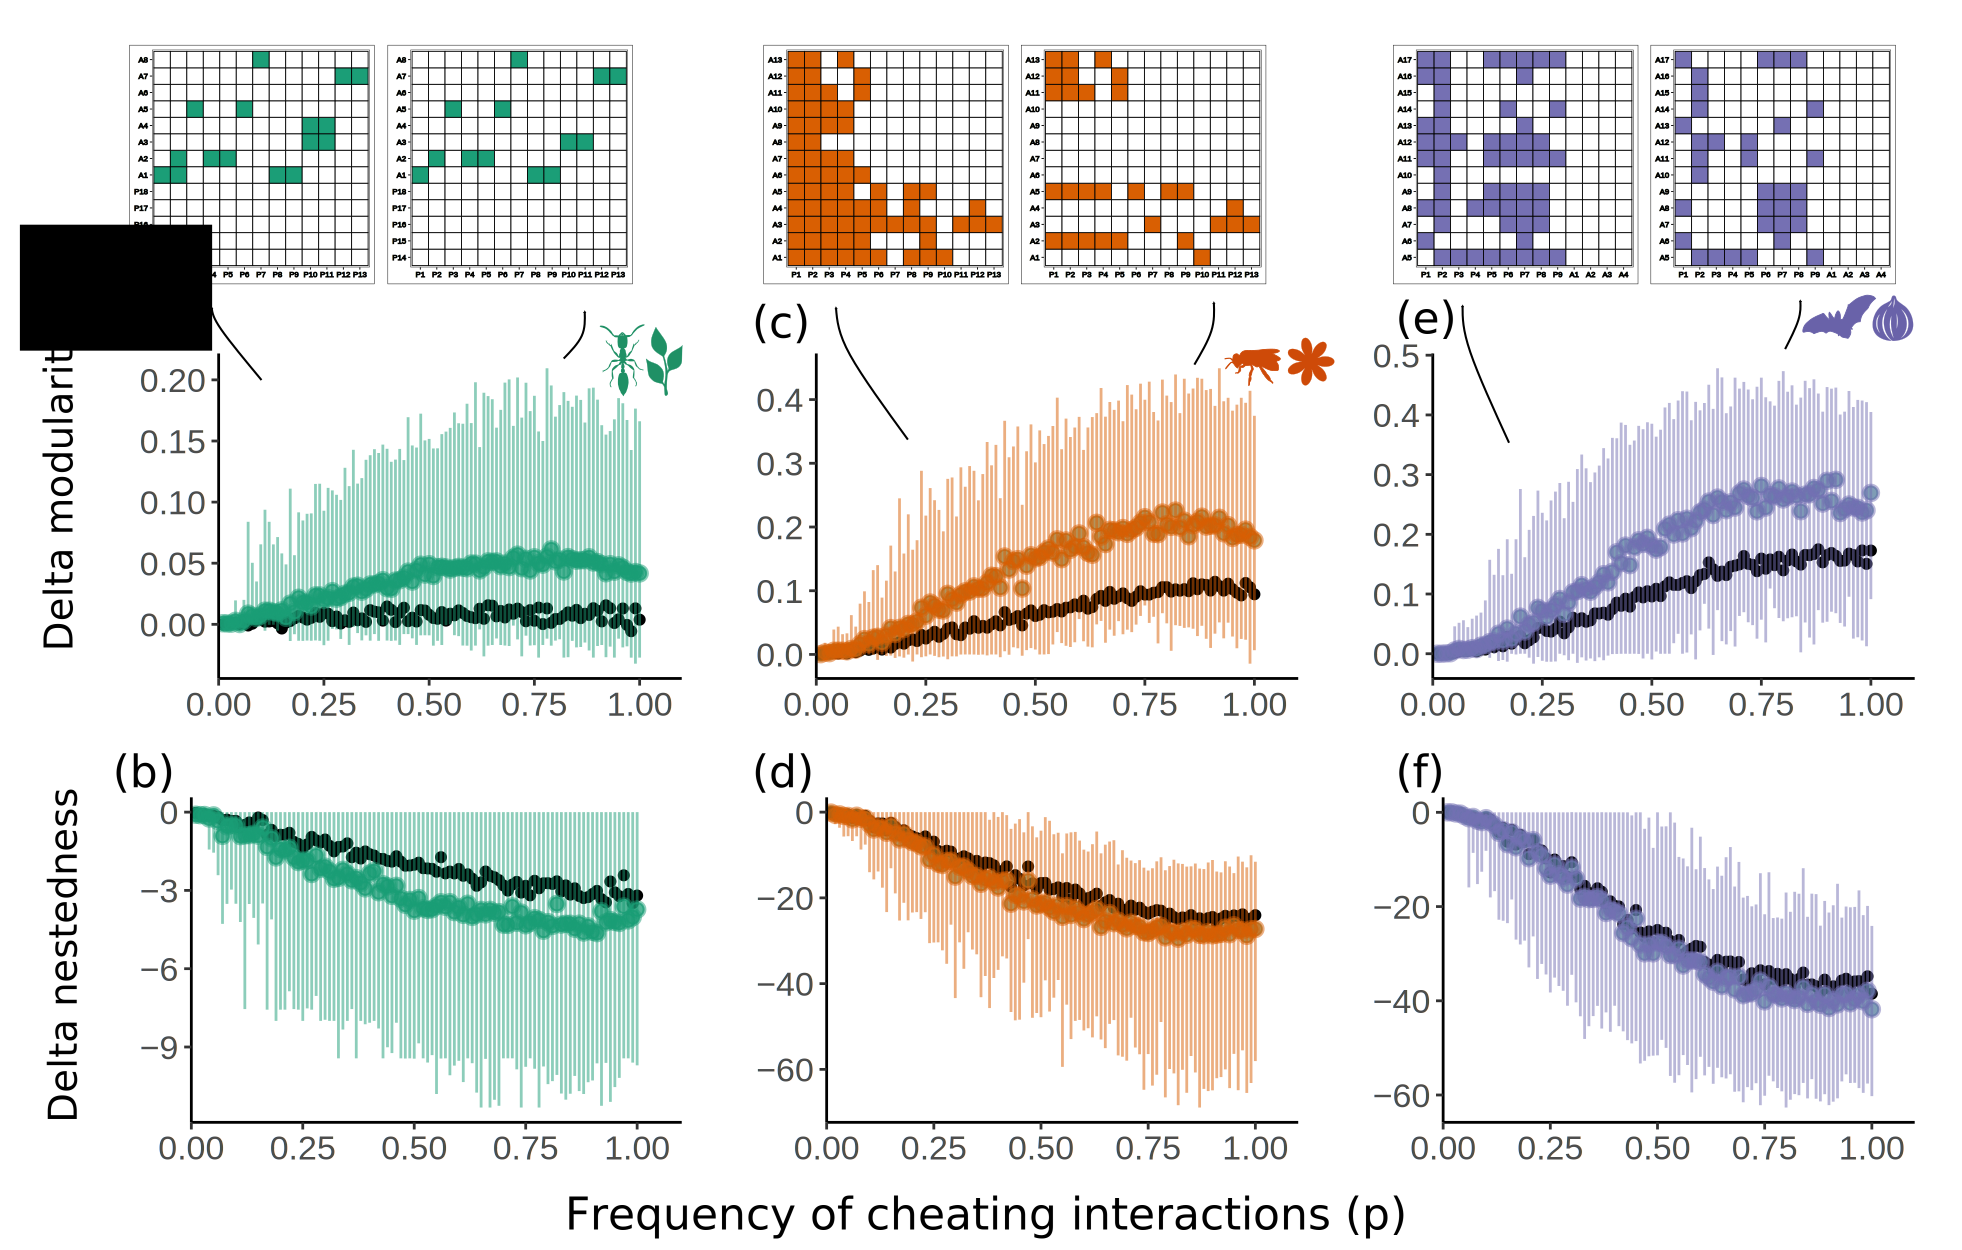
\includegraphics[width=\linewidth]{New_Figura_4.pdf}
  \vspace*{-7mm}
  \caption{Frequency of exploitation interactions modifies the structure of mutualistic networks through coevolution. The mutualistic networks tend to become more modular and less nested as we increase the frequency of exploitation interactions in the network. In ant-plant mutualisms, the networks are initially more modular than seed dispersal and pollination. Thus, the ant-plant networks undergo less structural changes than seed dispersal and pollination. Ant-plant interactions are represented by the green graphs, pollination by orange graphs and seed dispersal interactions are represented by purple graphs. The black points are parallel simulations where we zeroed interactions randomly.}
  \label{fig:4}
\end{figure}
\end{singlespace}

\begin{table}[H]
\caption{\label{tab:1}Variables and parameters of the model and their baseline values.}
\centering
\begin{adjustbox}{width=\columnwidth,center}
\resizebox{\textwidth}{!}{%
\begin{tabular}{ccc}
\hline
\textbf{Parameter} & \textbf{Description}                                                                                                             & \textbf{Baseline values} \\ \hline
$Z_{i}$            & Initial mean trait value \textit{Z} of species \textit{i}                                                                   & $Z_{i} \sim U(0, 10)$               \\
$\varphi_{i}$              & Parameter composed of the additive genetic variance and slope of adaptive landscape of \textit{Z}                       & 0.2        \\
$\varepsilon_{ij}$              & Trait barrier to happen the exploitation interaction between species  \textit{i} and \textit{j} & 5          \\
$\gamma_{i}$             & Strength of abiotic selection for trait change of species \textit{i}                                            &  0.1        \\
$\theta_{i}$            & $Z_{i}$ optimum value for the environmental selection                                                                            & $\theta_{i} \sim U(0, 10)$                   \\
$\alpha$              & Sensitivity of evolutionary effect due to the trait matching between interacting species                                         & 0.2        \\
\textit{p}         & Probability of an positive effect become negative in a mutualistic network                                                       & $0.01 \leq p \leq 1$                      \\
\textit{b}         & Trait barrier for any interaction happen between species in the network                                                          & 7          \\ \hline
\end{tabular}}
\end{adjustbox}
\end{table}

\begin{table}[H]
\caption{\label{tab:2}Average and standard deviation of $\Delta Q$ and $ \Delta NODF$ for random interaction removal and trait barrier interaction removal for three types of mutualisms}
\centering
\begin{adjustbox}{width=\columnwidth,center}
\resizebox{\textwidth}{!}{%
\begin{tabular}{lllll}
\hline
                       &\textbf{ $\Delta Q$ - Random removal}                                      & \textbf{$\Delta Q$ - Trait barrier removal}                               & \textbf{$\Delta NODF$- Random removal }                                    &\textbf{$\Delta NODF$- Trait barrier removal}                            \\ \hline
\textbf{Ant-Plant (n = 8)}      & $0.007 \pm 0.035$ & $0.037 \pm 0.056$ & $-1.65 \pm 2.52$   & $-2.96 \pm  3.39$ \\
\textbf{Pollination (n = 8)}    & $0.058 \pm  0.072$ & $0.14 \pm  0.12$   & $-14.9 \pm  13.5$   & $-19.4 \pm 15.4$ \\
\textbf{Seed dispersal (n = 8)} & $0.095 \pm 0.081$ & $0.18 \pm  0.14$   & $-23.06 \pm 17.02$ & $-26.3 \pm  19.0$ \\
\hline
\end{tabular}}
\end{adjustbox}
\end{table}

\nocite{aizen_when_2014}
\nocite{almeida-neto_consistent_2008}
\nocite{anderson_geographical_2008}
\nocite{andreazzi_network_2017}
\nocite{andreazzi_coevolution_2019}
\nocite{aubier_positive_nodate}
\nocite{banos-villalba_seed_2017}
\nocite{bascompte_plant-animal_2007}
\nocite{bastolla_architecture_2009}
\nocite{blanco_internal_2016}
\nocite{blondel_fast_2008}
\nocite{bronstein_exploitation_2001}
\nocite{bronstein_ecological_2003}
\nocite{burns_what_2013}
\nocite{ciampaglio_detecting_2001}
\nocite{dattilo_structure_2014}
\nocite{dodds_interspecific_1997}
\nocite{fernandes_coevolution_2019}
\nocite{ferriere_regis_cheating_2002}
\nocite{fontaine_ecological_2011}
\nocite{fouks_pollinator_2019}
\nocite{futuyma_coevolution_1983}
\nocite{galetti_functional_2013}
\nocite{genini_julieta_cheaters_2010}
\nocite{gilarranz_effects_2017}
\nocite{gomez_synzoochory:_2018}
\nocite{gonzalez-castro_relative_2015}
\nocite{guimaraes_jr_evolution_2011}
\nocite{herrera_long-term_1998}
\nocite{jordano_angiosperm_1995}
\nocite{jordano_invariant_2003}
\nocite{kauffman_coevolution_1991}
\nocite{lambers_life_2008}
\nocite{lande_natural_1976}
\nocite{law_mutualists_2001}
\nocite{lee_inherent_2015}
\nocite{melian_diversity_2009}
\nocite{mello_modularity_2011}
\nocite{montesinos-navarro_network_2017}
\nocite{newman_networks_2018}
\nocite{nuismer_coevolutionary_2005}
\nocite{nuismer_coevolution_2013}
\nocite{nuismer_gene_1999}
\nocite{olesen_modularity_2007}
\nocite{parchman_diversifying_2002}
\nocite{ponisio_coevolution_2017}
\nocite{rezende_effects_2007}
\nocite{rodriguezrodriguez_functional_2017}
\nocite{santamaria_linkage_2007}
\nocite{sauve_stability_2016}
\nocite{siepielski_conflicting_2010}
\nocite{song_towards_2020}
\nocite{stang_asymmetric_2007}
\nocite{thebault_stability_2010}
\nocite{thompson_coevolutionary_1994}
\nocite{thompson_geographic_2005}
\nocite{thompson_geographic_2002}
\nocite{tibshirani_estimating_2001}
\nocite{valientebanuet_beyond_2015}
\nocite{vieira_fruit_2003}
\nocite{ward_hierarchical_1963}
\nocite{wilson_coexistence_2003}
\nocite{zhang_adaptive_2013}

\addcontentsline{toc}{subsection}{References}
\subsection*{References}
\begin{singlespace}
\printbibliography[heading = none]
\end{singlespace}
\newpage

\addcontentsline{toc}{section}{Supplemental Informations}
\newrefsection
\renewcommand{\theequation}{S.\arabic{equation}}
\setcounter{equation}{0}
\section*{Supplemental Informations}

\addcontentsline{toc}{subsection}{Coevolution model}
\subsection*{Coevolution model}
Based on a classical approach of modeling trait changes by directional evolution (Lande 1976) and coevolutionary network models (Guimarães \textit{et al.} 2017, Andreazzi \textit{et al.} 2017), we used a mean-field approach to describe how an average quantitative trait $Z_{i}$ from a population changes in time due to selective pressures of mutualism, exploitation interactions, and other environmental selection sources. We assume that populations are large, resulting in negligible genetic drift. The classical approach to study single trait change are based on the Equation S1:

\begin{equation}  \label{supeq:1}
  \Delta z^{(t)}_{i} = h^{2}_{i} \sigma^{2}_{i} \frac{\partial{ln \overline{W}_{i}}}{\partial z^{(t)}_{i}}
\end{equation}

which $h^{2}_{i}$ is the trait heritability, $\sigma^{2}_{i}$ is the phenotypic trait variance and $\frac{\partial{ln \overline{W}_{i}}}{\partial z^{(t)}_{i}}$ is the selection gradient which defines the adaptive landscape of $z$ describing how the population average fitness $\overline{W}_{i}$ changes due to small variation in $z^{(t)}_{i}$. We assumed fixed trait heritability and phenotypic variance as simplifying assumptions. We described changes of average traits of a single population of a given species in time due to the selection gradient. The selection gradient, in turn, respond, primarily, to ecological interactions, such as mutualisms and exploitative interactions based on mutualism, but also to other selective pressures in the environment, such as low resource disponibility, climatic changes or human impact like defaunation and deforestation. We are considering a linear selection gradient which is defined as $\frac{\partial{ln \overline{W}_{i}}}{\partial z^{(t)}_{i}} = \rho_{i}(z_{i, p} - z^{(t)}_{i})$ where $\rho_{i}$ is a constant defining the sensitivity of $\overline{W}_{i}$ due to small changes in $z^{(t)}_{i}$ in time and $z_{i, p}$ is the adaptive peak for species \textit{i}.

In our approach, the adaptive peak $z_{i, p}$ is different depending on the interaction effect that the species \textit{i} has with a certain species \textit{j}. Positive effects (\textit{+}) affecting the species \textit{i} from mutualistic interactions (\textit{++}) and from a species exploiting a victim (\textit{+-}) will favour the adaptive peak called $z_{i, p +}$ described in Equation S2 favouring the species trait matching. However, selection on an victim species \textit{i} which has a negative effect (\textit{-}) from interact with the exploiter species \textit{j} will favour the adaptive peak $z_{i, p -}$ described in the Equation S3:

\begin{equation}  \label{supeq:2}
  z_{i, p +} = \sum_{j, j \neq i}^{N} (1 - \gamma_{i})(x^{(t)}_{ij} m^{(t)}_{ij}) + \gamma_{i} \theta_{i}
\end{equation}

\begin{equation} \label{supeq:3}
  z_{i, p -} = \sum_{j, j \neq i}^{N}(1 - \gamma_{i})[(x^{(t)}_{ij} \pm \varepsilon_{ij})(\delta_{ij})v^{(t)}_{ij})] + \gamma_{i} \theta_{i}
\end{equation}

and showed in Sup.Figure 1, where $x^{(t)}_{ij}$ is the mean trait value of species \textit{i} favoured by the interaction with species \textit{j}, $\varepsilon_{ij}$ is the trait barrier which imposes a minimum trait matching between species to have an evolutionary effect between the exploiter and the victim, $\gamma_i$ is the proportional importance of the environmental selection to trait changes and $\theta_i$ is the optimum trait value favoured by the environmental selection. The adaptive peak $ z_{i, p -}$ has an operator $\delta_{ij}$ which dictates if the adaptive peak will change given the trait differences between \textit{i} and \textit{j}. If the trait difference between \textit{i} and \textit{j} is higher than the barrier $\varepsilon_{ij}$, then $\delta_{ij} = 0$, see S4 below. If the victim and the exploiter are sufficiently similar, the change in the adaptive peak will follow the conditions showed in S5, increasing or decreasing the adaptive peak value depending on the absolute difference between $x^{(t)}_{ij}$ and $z_{i}$:

\begin{equation} \label{supeq:4}
\abs{x^{(t)}_{ij} \pm \varepsilon_{ij} - z_{i}} < \abs{x^{t}_{ij} - z_{i}} \implies \delta_{ij} = 0
\end{equation}

\begin{equation} \label{supeq:5}
    \systeme*{\abs{x^{(t)}_{ij} > z_{i}} \implies \delta_{ij} = 1 \implies x^{(t)}_{ij} + \varepsilon_{ij},\abs{x^{(t)}_{ij} < z_{i}} \implies \delta_{ij} = 1 \implies x^{(t)}_{ij} - \varepsilon_{ij}}
\end{equation}

Finally, by assuming (\textit{i}) $x^{(t)}_{ij} = z^{(t)}_{j}$ which defines the trait matching between \textit{i} and \textit{j}; (\textit{ii}), $\varphi_{i}$ is fixed and it is a composed parameter that combines the additive genetic variance of $z_{i}$ and the slope of the selection gradient, $\varphi_{i} = \rho_{i} \sigma^{2}_{G_z}$ and; (\textit{iii}) combining  S1, S2 and S3 we obtain the Equation 5 from the main text

\begin{equation} \tag{5}
  Z^{(t+1)}_{i} = Z^{(t)}_{i} + \varphi_{i}\{(1 - \gamma_{i})[\sum_{j} m^{(t)}_{ij}(Z^{(t)}_{j} - Z^{(t)}_{i}) + \sum_{j}\delta_{ij}v^{(t)}_{ij}(Z^{(t)}_{j} \pm \varepsilon_{ij} - Z^{(t)}_{i})] + \gamma_{i}(\theta_{i} - Z^{(t)}_{i})\}
\end{equation}

which $m^{(t)}_{ij}$ and $v^{(t)}_{ij}$ components are the evolutionary effects of species \textit{j} on \textit{i} weighted by all the other effects that \textit{i} has with other species in the community. We separate positive and negative effects in single interaction matrices, associating each effect with their proper network. The evolutive effects of mutualism $m^{(t)}_{ij}$ and exploitative $v^{(t)}_{ij}$ come from the same evolutive effects matrix named \textbf{Q}. The elements of \textbf{Q} are described as the partial effect of species \textit{j} in species \textit{i} $e^{-\alpha(Z^{(t)}_{j} - Z^{(t)}_{i})^2}$ normalized by the sum of all other effects between \textit{i} and all his partners \textit{k} $\sum_{k, i \neq k} e^{-\alpha(Z^{(t)}_{k} - Z^{(t)}_{i})^2}$  with $\alpha$ being the sensitivity parameter that control the intensity of the effect due to how similar are the traits. Putting both these equations together we define $q^{(t)}_{ij}$ which is the partial evolutionary effects of species \textit{i} and \textit{j} in the community as shown in the Equation S6:

\begin{equation} \label{supeq:6}
  q^{(t)}_{ij} = \frac{e^{-\alpha(Z^{(t)}_{j} - Z^{(t)}_{i})^2}}{\sum_{k, i \neq k} a_{ik} e^{-\alpha(Z^{(t)}_{k} - Z^{(t)}_{i})^2} }
\end{equation}

Finally, we have $m^{(t)}_{ij}$ and $v^{(t)}_{ij}$ using the $q^{(t)}_{ij}$ with the $A_{m}$ or $A_{v}$ depending on the interaction, mutualism or exploitative, between \textit{i} and \textit{j} like shown in Equation S7 and S8:

\begin{equation} \label{supeq:7}
  m^{(t)}_{ij} = A_{m_{ij}}q^{(t)}_{ij}
\end{equation}

\begin{equation} \label{supeq:8}
  v^{(t)}_{ij} = A_{v_{ij}}q^{(t)}_{ij}
\end{equation}

\addcontentsline{toc}{subsection}{Networks characterization}
\subsection*{Networks characterization}
Understanding the effect of exploitation in species coevolution in mutualistic networks requires a structural quantification of networks, allowing predictions about whether a network structural pattern will change, and if so, how they change. For that, we combine classic algorithms and graph theory definitions to characterize our networks. Considering that a single binary matrix of interactions called \textbf{A} has a number of animals equal to $N_{A}$ and the number of plants $N_{P}$, the richness \textit{N} of the community will be $N_{A}+N_{P}$. Each of those species has a number of interactions, which we called species degree (\textit{k}). Using the binary matrix, we calculated \textit{k} for species \textit{i} as the row sums of line \textit{i} $\sum_{1}^{N}a_{i}$. Considering that we have two layers for a single bipartite network, we can use the same approach in each layer to have the degree of positive effects for species \textit{i} $\sum_{1}^{N}A_{m_{i}}$ and negative effects $\sum_{1}^{N}A_{v_{i}}$ which in this case, $m_{i}$ and $v_{i}$ are the elements of row \textit{i} in the networks $A_{m}$ and$A_{v}$. The connectance \textit{L}  is a measure of the proportion of the realized interactions in the network which is defined in Equation S9:

\begin{equation} \label{supeq:9}
  L = \frac{\sum_{i}^{N_{A}}\sum_{j \neq i}^{N_{P}}a_{ij}}{N_{A}N_{P}}
\end{equation}

Modularity \textit{Q} can be defined as the difference of a fraction of interactions within a module and the expected number of interactions in that module by chance (Blondel \textit{et al.} 2008) as shown in equation S10: 

\begin{equation} \label{supeq:10}
  Q = \frac{1}{2m} \sum_{ij}(A_{ij} - \frac{k_{i}k_{j}}{2m}) \delta(c_{i}, c_{j})
\end{equation}

which \textit{m} is half the total number of observed links in the network, $A_{ij}$ is the element of the binary adjacency matrix, $k_{i}$ is the degree for each link and $\delta(c_{i}, c_{j}) = 1$ indicates if \textit{i} and \textit{j} are in the same module and $\delta(c_{i}, c_{j}) = 0$ otherwise. The \textit{Q} metric for modularity ranges from -1 which represents minimum modularity to 1; maximum modularity. We use an algorithm created by Blondel \textit{et al.} 2008 which iteratively optimizes the modularity of the network changing nodes position to maximize modularity. Using these new networks with swapped nodes, the algorithm constructs a meta network finding the best global modularity value for the initial network. Finally, nestedness is a measure of how much the interactions of specialists is a subset of the interactions from a core of generalist calculated with a metric called \textit{NODF} (Almeida-Neto \textit{et al.} 2008) which is calculated as shown in S11:

\begin{equation} \label{supeq:11}
  NODF = \frac{\sum_{N_{paired}}}{(\frac{N_{A}(N_{A} - 1)}{2}) + (\frac{N_{P}(N_{P} - 1)}{2})}
\end{equation}

which $N_{paired}$ is a measure of overlap defined as the percentage of interactions in a given column to a given row. The \textit{NODF} metric ranges from 0, non nestedness to 100; fully-nested network. The Sup.Table 1 contains all those metrics for each of our empirical networks of interactions used in our simulations.

\renewcommand{\thetable}{S\arabic{table}}
\setcounter{table}{0}
\begin{table}[H]
\caption{\label{suptab:1}24 Empirical networks used to parametrize our numerical simulations. We have eight networks for each type of mutualism (Pollination, Seed Dispersal and Ant-Plant) varying in species richness (\textit{N}), connectance (\textit{L}), modularity (\textit{Q}) and nestedness (\textit{NODF})}
\centering
\begin{adjustbox}{width=\columnwidth,center}
\resizebox{\textwidth}{!}{%
\begin{tabular}{|l|l|l|l|l|l|l|l|}
\hline
\multicolumn{1}{|c|}{\textbf{Net}} & \multicolumn{1}{c|}{\textbf{Type}} & \multicolumn{1}{c|}{\textbf{N}} & \multicolumn{1}{c|}{\textbf{L}} & \multicolumn{1}{c|}{\textbf{Q}} & \multicolumn{1}{c|}{\textbf{NODF}} & \multicolumn{1}{c|}{\textbf{Location}} & \multicolumn{1}{c|}{\textbf{Reference}} \\ \hline
1                                  & Pollination                        & 26                              & 0.42                            & 0.17                            & 84.93                              & Brazil                                 & Bezerra \textit{et al.} 2009                             \\ \hline
2                                  & Pollination                        & 30                              & 0.23                            & 0.36                            & 42.72                              & Canadá                                 & Mosquin \& Martin 1967                                   \\ \hline
3                                  & Pollination                        & 27                              & 0.28                            & 0.28                            & 51.87                              & Mauritius                              & Olesen \textit{et al.} 2012                              \\ \hline
4                                  & Pollination                        & 22                              & 0.25                            & 0.43                            & 35.96                              & Portugal                               & Olesen \textit{et al.} 2012                             \\ \hline
5                                  & Pollination                        & 39                              & 0.14                            & 0.53                            & 29.53                              & Argentina                              & Vázquez \& Simberloff 2003                      \\ \hline
6                                  & Pollination                        & 42                              & 0.15                            & 0.60                            & 18.65                              & Argentina                              & Vázquez \& Simberloff 2003                      \\ \hline
7                                  & Pollination                        & 39                              & 0.14                            & 0.56                            & 26.31                              & Argentina                              & Vázquez \& Simberloff 2003                       \\ \hline
8                                  & Pollination                        & 34                              & 0.17                            & 0.54                            & 23.27                              & Argentina                              & Vázquez \& Simberloff 2003                       \\ \hline
9                                  & Seed dispersal                     & 28                              & 0.34                            & 0.28                            & 50.98                              & USA                                    & Baird 1980                                      \\ \hline
10                                 & Seed dispersal                     & 40                              & 0.42                            & 0.20                            & 67.66                              & Papua New Guinea                       & Beehler 1983                                    \\ \hline
11                                 & Seed dispersal                     & 36                              & 0.16                            & 0.42                            & 34.16                              & Puerto Rico                            & Carlo \textit{et al.} 2003                               \\ \hline
12                                 & Seed dispersal                     & 33                              & 0.44                            & 0.22                            & 78.75                              & Spain                                  & Jordano 1985                                    \\ \hline
13                                 & Seed dispersal                     & 32                              & 0.63                            & 0.15                            & 67.34                              & México                                 & Kantak 1979                                     \\ \hline
14                                 & Seed dispersal                     & 23                              & 0.43                            & 0.32                            & 48.29                              & Panamá                                 & Poulin \textit{et al.} 1999                              \\ \hline
15                                 & Seed dispersal                     & 24                              & 0.37                            & 0.22                            & 73.89                              & Panamá                                 &Poulin \textit{et al.} 1999                              \\ \hline
16                                 & Seed dispersal                     & 26                              & 0.27                            & 0.30                            & 42.70                              & United Kingdom                         &Sorensen 1981                                  \\ \hline
17                                 & Ant-Plant                          & 11                              & 0.23                            & 0.69                            & 8                                  & Brazil                                 & Thiago Izzo, unpublished data                   \\ \hline
18                                 & Ant-Plant                          & 16                              & 0.17                            & 0.77                            & 7.01                               & Brazil                                 & Thiago Izzo, unpublished data                   \\ \hline
19                                 & Ant-Plant                          & 21                              & 0.16                            & 0.68                            & 11.32                              & Brazil                                 & Thiago Izzo, unpublished data                   \\ \hline
20                                 & Ant-Plant                          & 15                              & 0.16                            & 0.79                            & 0                                  & Brazil                                 & Thiago Izzo, unpublished data                   \\ \hline
21                                 & Ant-Plant                          & 21                              & 0.14                            & 0.78                            & 4.90                               & Brazil                                 & Thiago Izzo, unpublished data                   \\ \hline
22                                 & Ant-Plant                          & 18                              & 0.15                            & 0.77                            & 4.10                               & Peru                                   & Thiago Izzo, unpublished data                   \\ \hline
23                                 & Ant-Plant                          & 26                              & 0.13                            & 0.77                            & 3.49                               & Brazil                                 & Davidson \& Fisher 1991                         \\ \hline
24                                 & Ant-Plant                          & 41                              & 0.12                            & 0.64                            & 13.63                              & Brazil                                 & Fonseca \& Ganade 1996                          \\ \hline
\end{tabular}}
\end{adjustbox}
\end{table}

\addcontentsline{toc}{subsection}{Interaction shift}
\subsection*{Interaction shifts}
Here, we used a multiplex network approach, a special case of a multilayer network in which the nodes represent the same set of species in different layers (Newman 2018). Using two layers of a single bipartite adjacency matrix of interactions \textbf{A}, one for the positive effects \textbf{Am} and another for the negative effects \textbf{Av}, we can define species which do not have an unique role in the community but can act as a mutualist or an exploiter in the same community (Genrich \textit{et al.} 2017). The adjacency matrix layer called \textbf{Am} have the animals and the plants placed in the columns and in the rows, respectively. This \textbf{Am} matrix holds the positive effects in the community, when $A_{m_{ij}} = 1; A_{m_{ji}} = 1$ a mutualistic interaction happens between \textit{i} and \textit{j} and $A_{m_{ij}} = 0; A_{m_{ji}} = 0$ the interaction did not happen. Accordingly, the negative effects we have in an adjacency matrix layer \textbf{Av} with the same rows and columns as \textbf{Am} but representing the presence/absence of negative effects. This exploitation interactions are defined as a positive effect of species \textit{j} in \textit{i} ($A_{m_{ij}} = 1; A_{v_{ji}} = 0$) but a negative effect of \textit{i} in \textit{j}  ($A_{m_{ji}} = 0; A_{v_{ji}} = 1$). Thus, we have two complementary bipartite adjacency matrices layers which represents the formation of a mutualistic interaction or an exploitation depending on how species are affecting each other.

The insertion of exploitation interactions in mutualistic networks depends on a certain probability \textit{p} that an interaction shifts to a positive to a negative effect. In our simulations, \textit{p} is equal in every element in the \textbf{Am} matrix. Based on \textit{p}, we pass the positive effects between the species from the \textbf{Am} to \textbf{Av} matrix. Thus, the element $A_{m_{ij}}$ will pass from 1 to 0 in the \textbf{Am} matrix and the element $A_{v_{ji}}$ will pass from 0 to 1 in the \textbf{Av} matrix. For test if the value of \textit{p} is a good approximation of the frequency of negative effects in the network, we can calculate the expected frequency of exploitation interactions in any network, here called as $f_{Ch}$ which we expect that $p =f_{Ch}$ as shown in Sup.Figure 2. With that, we can have higher frequency of exploiting interactions in networks with higher values of \textit{p}. With this approach we explore novels coevolutionary dynamics, where the presence of exploitative interactions changes the species trait matching and the network structure in mutualistic networks (Sup.Figure 3).

In the main text,  we argued  that the definition of the maximum timesteps were enough to describe equilibria in different simulations. We run additional simulations to test if, in 1000 timesteps, we reach  our stop simulation criterium $\abs{Z^{(t+1)}_{i} - Z^{(t)}_{i}} < 10^{-4}$ to any species \textit{i}. As shown in Sup.Figure 4, the simulations usually stops before the $10^{-4}$ timesteps. We also test if the stop simulations criteria based on difference of traits influences our trait matching metrics, running simulations with minimum values of $\abs{Z^{(t+1)}_{i} - Z^{(t)}_{i}}$ fixed on $10^{-8}$; $10^{-6}$ and $10^{-4}$. The Sup.Figure 5 shows that different critical values of $\abs{Z^{(t+1)}_{i} - Z^{(t)}_{i}}$ do not affect the \textit{MPD} but has an impact in the clustering of species traits. Finally, a fundamental model assumption is that the interaction shifts from mutualism to exploitation occurs before, and not during the coevolution process. This assumption is a first step  to explore the outcomes changes in ecological communities, but it is possible the interaction outcomes change during the coevolutionary process in natural communities. We perform a set of simulations in which we allowed outcomes shifts during the simulations. The outcomes shifts depends on a secondary probability called \textit{g} ranging from 0.01 to 1. Thus, higher values of \textit{g} generates higher outcomes shifts during the simulations. If in a certain timestep \textit{t} an interaction outcome shift, we randomly sample two effects to change. First, we sample an positive effect and transform it into negative ($A_{m_{ij}} = 0; A_{v_{ij}} = 1$) and a negative effect into positive ($A_{m_{kl}} = 1; A_{v_{kl}} = 0$, which $ k \neq i; l \neq j$). Changing two effects when an outcome shift happens in time allow maintain the \textit{p} value fixed, changing only the interaction outcome organization of the network. However there could be cases which there are none positive or negative effects enough to shift two effects in a single timestep, \textit{i.e.}, simulations with extreme values of \textit{p}. In that cases, a single effect is changed in that timestep. Having said that, we imposed that in the next interaction shift  an change in the opposite direction will occur, avoiding creating long-term bias in \textit{p}. The Sup.Figure 6 shows our trait matching metrics from simulations in scenarios with different values of \textit{p} and \textit{g} using a theoretical fully connected bipartite network showing no differences in our main result when we considerer interactions shifts during the simulations.

\addcontentsline{toc}{subsection}{Trait clustering analisys}
\subsection*{Trait clustering analysis}
The differences in the adaptive peak for positive and negative effects raises a question on how the interplay between these adaptive peaks drives the species trait matching. We calculated the Euclidean distance between species traits generating an distance matrix which was used to perform an hierarchical clustering analysis called Ward's method (Ward 1963). This method was chosen because it minimizes the within-cluster variance as merge species in clusters of similar traits, \textit{i.e.} form clusters of species with high trait matching compared to others species.

Together with the Ward's method we performed cluster validation analysis which return the optimized number of clusters formed by \textit{N} species, thus the maximum number of clusters is equal to \textit{N-1}. This optimized number of clusters is considered as the number of clusters formed due to coevolution process and was used to explore the cluster formation with different values of \textit{p} in main text; \textbf{Figure 2} and \textbf{Figure 3}. We used the \textit{GAP} algorithm which compares different numbers of clusters in our data with a null distribution, returning the optimized number of clusters which the null distribution most failed to create (Tibshirani \textit{et al.} 2001). Thus, the minimal number of species trait cluster is 2. All the clustering analysis was made using the NbCluster R package (Charrad \textit{et al.} 2014). 

\renewcommand{\thefigure}{S\arabic{figure}}
\setcounter{figure}{0}  

\addcontentsline{toc}{subsection}{Figures and tables}
\subsection*{Figures and tables}

\begin{singlespace}
\begin{figure}[H]
  \centering
  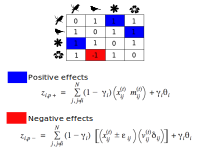
\includegraphics[width=\linewidth]{Sup_Figura_1.pdf}
  \vspace*{-7mm}
  \caption{Each effect between interacting species (\textit{+} or \textit{-}) in a community represented by an adjacency matrix of interactions are described by an adaptive peak. Each peak is influenced by the environmental factors of importance \textit{i} favouring a trait value called \textit{i} and the ecological interactions which the positive effects favoured the species trait matching and the negative effect the trait decoupling due to the $\varepsilon_{ij}$. Finally, the sum of all the effects (positive and negatives) for a single species defines the final adaptive peak for that species (S2 and S3).}
  \label{supfig:1}
\end{figure}

\begin{figure}[H]
 \centering
  \includegraphics[width=\linewidth]{Sup_Figura_2.pdf}
  \vspace*{-7mm}
  \caption{Consistency test of expected frequency of exploitation interactions in a fully connected bipartite network with 50 species. For \textit{p} ranging from 0.01 to 1, we plot the expected and observed value of frequency of negative effects in the network. The expected frequency it's simply the value of \textit{p} used and the observed values are the frequency of interactions in the \textbf{Av} matrix. The value of \textit{p} used is a good proxy for the frequency of exploitation interactions in networks $f_{Ch}$.}
  \label{supfig:2}
\end{figure}

\begin{figure}[H]
 \centering
  \includegraphics[width=\linewidth]{Sup_Figura_3.pdf}
  \vspace*{-7mm}
  \caption{Four theoretical examples of coevolutionary dynamics showing \textit{Z}, the mean trait values of 10 species described by our main model in a theoretical fully connected bipartite adjacency matrix with different values of frequency of exploitation interactions $f_{Ch}$ inserted in a mutualistic network. Each graph is a single simulation where we show the increase in trait disparity and the gradual formation of species traits aggregation as we insert a higher quantity of negative effects in a mutualistic network, drawing attention to the Y axis scale in the $f_{Ch} = 0.8$ graph.}
  \label{supfig:3}
\end{figure}

\begin{figure}[H]
 \centering
  \includegraphics[width=\linewidth]{Sup_Figura_4.png}
  \vspace*{-7mm}
  \caption{Number of timesteps to reach the equilibrium condition. Each line in the graph represents one of our 24 empirical adjacency matrix showing a density plot of 100 simulations for each of these networks. For each simulation we compute the time to reach the equilibrium and get an density line showing the distribution of simulations timesteps. Despite the fact that a considerable number of simulations follows to 1.000 timesteps, the majority of this simulations ends at 300-500 timesteps.}
  \label{supfig:4}
\end{figure}

\begin{figure}[H]
 \centering
  \includegraphics[width = \linewidth, height = 17cm]{Sup_Figura_5.pdf}
  \vspace*{-7mm}
  \caption{Sensibility analysis showing our trait matching metrics with different equilibrium conditions to our simulations. Each point in the graph shows the \textit{MPD} and clustering of species traits in three different trait equilibrium values: $10^{-8}; 10^{-6}$ and $10^{-4}$. We have 100 simulations for each scenario totalizing 300 simulations.}
  \label{supfig:5}
\end{figure}

\begin{figure}[H]
 \centering
  \includegraphics[width = \linewidth, height = 17cm]{Sup_Figura_6.png}
  \vspace*{-7mm}
  \caption{The influence of the interaction shift during the simulations (controlling by \textit{g}, in rows) in the \textit{MPD} and clustering of species traits with different values of \textit{p}, in columns. There is a higher \textit{MPD} with the increasing of \textit{p} even if different probabilities of interaction shifts in time \textit{g}. The number of species trait clusters remain the same in all simulations. Each point in the graph is a coevolution simulation of a fully connected theoretical network with 50 species.}
  \label{supfig:6}
\end{figure}
\end{singlespace}

\newpage
\addcontentsline{toc}{subsection}{Code and data accessibility}
\subsection*{Code and data accessibility}
All the functions, scripts, results and figures used in the paper are available online in the GitHub platform in the \textit{coevo mut antag} repository. Additionally, you will find small guides and tutorials where we shown the basic process of simulation and how the main figures was generated. Also, we provide a link to the database's where all the empirical networks could be find and downloaded.

\begin{itemize}
    \item \href{https://github.com/lucascamacho/coevo_mut_antag}{GitHub repository}
    \item \href{http://www.web-of-life.es}{Web of Life website}
    \item \href{https://www.nceas.ucsb.edu/interactionweb/}{Interaction Web Data Base}
\end{itemize}

\nocite{almeida-neto_consistent_2008}
\nocite{andreazzi_network_2017}
\nocite{baird_selection_1980}
\nocite{beehler_frugivory_1983}
\nocite{bezerra_pollination_2009}
\nocite{blondel_fast_2008}
\nocite{carlo_avian_2003}
\nocite{charrad_nbclust_2014}
\nocite{davidson_symbiosis_1991}
\nocite{fonseca_asymmetries_1996}
\nocite{genrich_duality_2017}
\nocite{guimaraes_jr_indirect_2017}
\nocite{jordano_ciclo_1985}
\nocite{kantak_observations_1979}
\nocite{lande_natural_1976}
\nocite{mosquin_observations_1967}
\nocite{newman_networks_2018}
\nocite{olesen_biodiversity_2012}
\nocite{poulin_interspecific_1999}
\nocite{sorensen_interactions_1981}
\nocite{tibshirani_estimating_2001}
\nocite{vazquez_changes_2003}
\nocite{ward_hierarchical_1963}

\addcontentsline{toc}{subsection}{References}
\begin{singlespace}
\subsection*{References}
\printbibliography[heading = none]
\end{singlespace}
\newpage

\end{document}